\newpage
\section{Frontend Architecture and S3 Deployment}

\subsection{Frontend Technology Stack and Compilation Pipeline}
The CloudCampus client tier is implemented as a single-page application (SPA) utilizing React 18.3.1, TypeScript 5.5.4, and TailwindCSS 3.4.9, bundled through Vite 5.4.0 \cite{vite_react}. The production build command (\texttt{npm run build}) triggers TypeScript type-checking followed by static bundle generation into the \texttt{frontend/dist/} directory:

\begin{itemize}[leftmargin=*,itemsep=1pt]
    \item \texttt{dist/index.html} (678 bytes): Root entry HTML loading application scripts and styles.
    \item \texttt{dist/assets/index-CkhRGeOg.css} (34.18 kB): Minified TailwindCSS design tokens and components.
    \item \texttt{dist/assets/index-BU0Jy3JJ.js} (766.84 kB): Minified and tree-shaken JavaScript runtime bundle.
\end{itemize}

\subsection{Amazon S3 Static Website Hosting \& Client Routing}
The compiled assets are hosted in the dedicated bucket \texttt{cloudcampus-frontend-production}. S3 Static Website Hosting is configured with \texttt{index.html} designated as both the Index Document and the Error Document. Because React Router DOM manages client-side routes (e.g., \texttt{/student/dashboard}, \texttt{/faculty/attendance}, \texttt{/admin/monitoring}), S3 routing rules redirect non-existent object keys back to \texttt{index.html} with HTTP 200, enabling uninterrupted SPA navigation.

\begin{figure}[H]
\centering
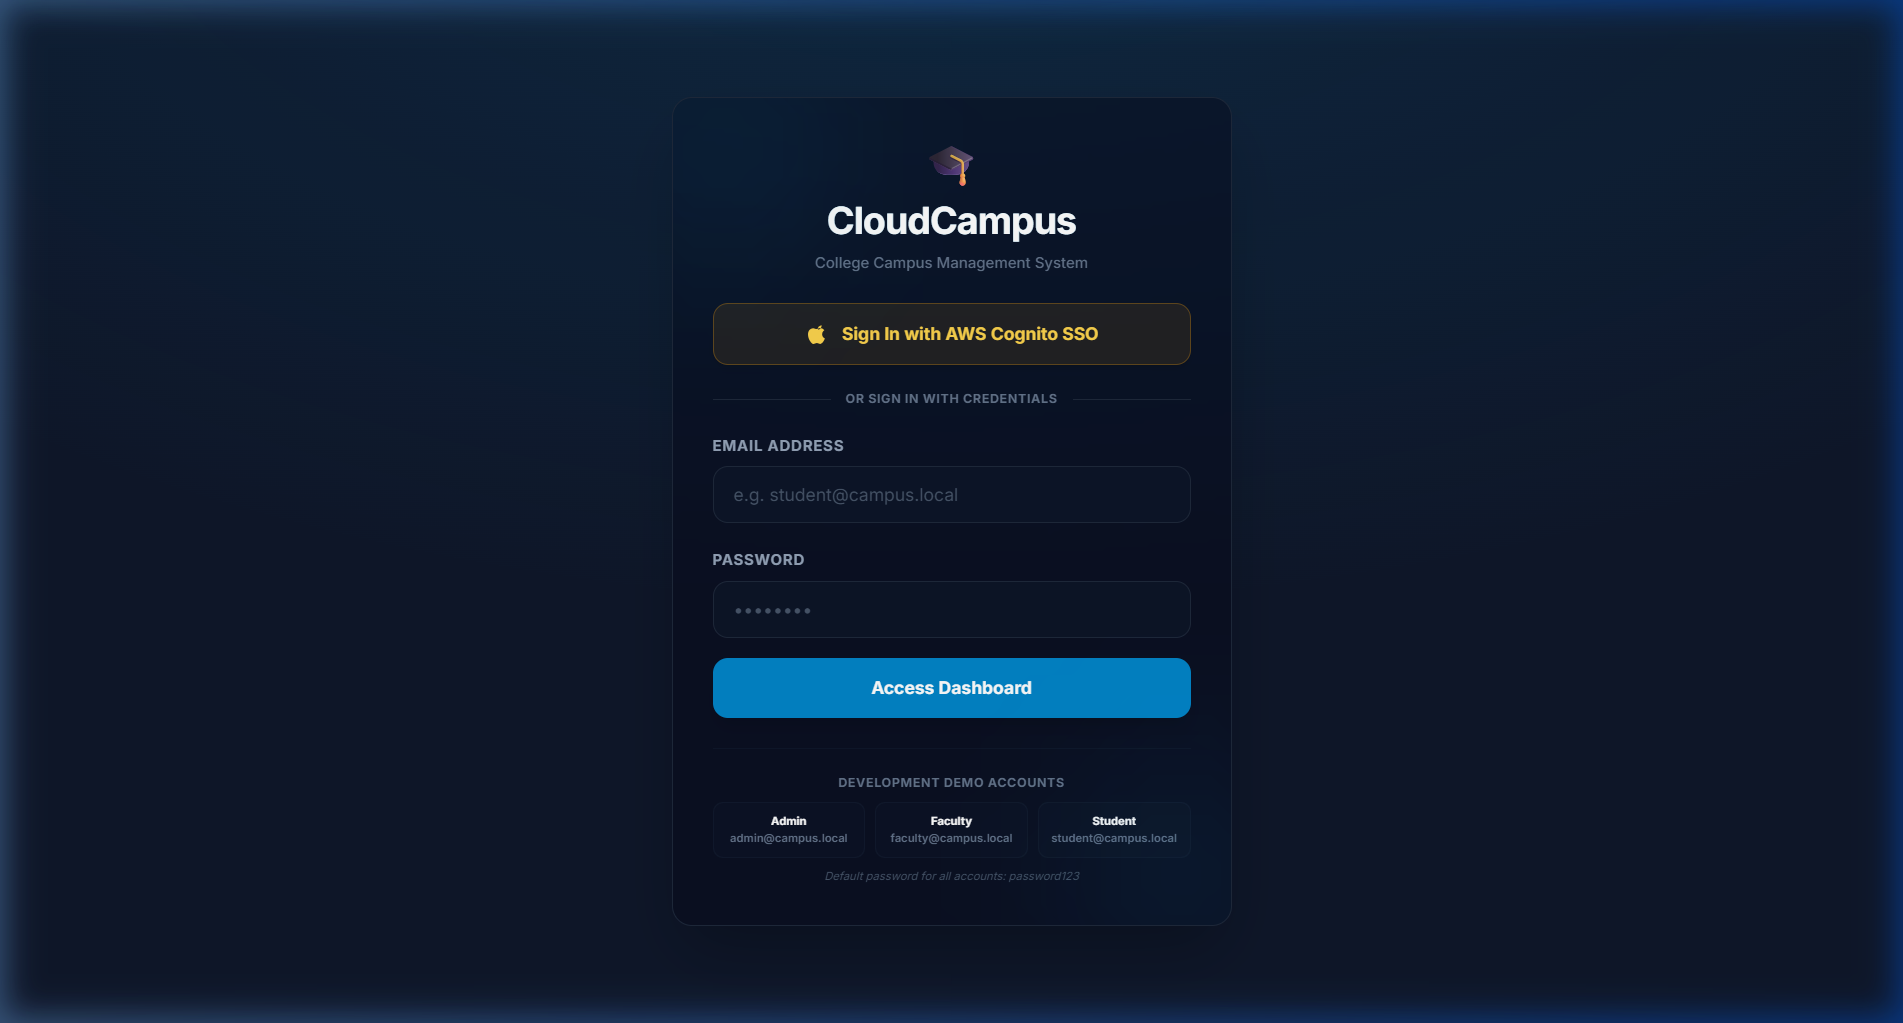
\includegraphics[width=0.88\textwidth]{assets/screenshots/browser/login_screen_1788353105637.png}
\caption{Live Production S3 Static Website Login Interface (\texttt{http://cloudcampus-frontend-production.s3-website-us-east-1.amazonaws.com})}
\label{fig:live_s3_frontend}
\end{figure}
